\documentclass[a4paper, 14pt, fleqn]{extarticle}
\usepackage{float}
\usepackage[justification=centering]{caption}
\usepackage{fefutitle}

\begin{document}
	\fefutitle{4}
	\pagebreak	

	\section{Введение}
		В данной лабораторной работе мне нужно решить и дать хар-ку линейных уравнений высших порядков, решить задачу Коши для уравнений 2-го порядка и
		найти коэффициент логистичекого уравнения.
	\pagebreak
	\section{Задание 1}
		\subsection{Постановка задачи}
			\noindent Для следующих линейных дифференциальных уравнений дать характеристику
					и найти общее решение:
		\begin{enumerate}
			\item \(y'' - y'\tan{x} - y\sec^2{x} = 0 \)
			\item \(y'' - y' = \tanh{x} \)	
			\item \(x^2y'' + 2xy' = \Big(2 + \ln^2{x}\Big)\cdot \sinh{(5\ln{x})} \cdot \sin{(\ln{x})} \)
			\item \(x^{\MakeUppercase{\romannumeral 4}} + 2x''' + 30x'' + 8x' + 104x = \big(-6 + 5t^2\big) \cdot \sinh{4t} \)
			\item \((x-1)^2y'' - x^2y' + 2xy = 2y'' -3y' + 2y \)
		\end{enumerate}
		\subsection{Решение}
			\noindent Поиск решения и построение векторного поля будет проводиться в системе компьютерной математики Wolfram Mathematica.
			\begin{enumerate}
				\item \(y'' - y'\tan{x} - y\sec^2{x} = 0 \)

					\textit{Характеристика:} Линейное однородное приведенное дифференциальное уравнения второго порядка с переменными коэффициентами
		
					\textit{Ответ:} \( y\cos{x} = C_1\sin{x} + C_2 \)

				\item \(y'' - y' = \tanh{x} \)	

					\textit{Характеристика:} Линейное неоднородное приведенное дифференциальное уравнения второго порядка с постоянными коэффициентами, неоднородность общего вида
		
					\textit{Ответ:} \( y = C_1 e^x + C_2 e^{-x} + (e^x + e^{-x}) \arctg{e^x} \)
				\pagebreak
				\item \(x^2y'' + 2xy' = \Big(2 + \ln^2{x}\Big)\cdot \sinh{(5\ln{x})} \cdot \sin{(\ln{x})} \)

					\textit{Характеристика:} Уравнение Эйлера второго порядка, характерестическая неоднородность после замены \( x = e^t \)
		
					\textit{Ответ:} \(\begin{aligned}[t] y &= \dfrac{C_1}{x} + C_2 + \dfrac{29x^5\ln^2{x}\cdot\sin{\ln{x}}}{1924} - \dfrac{19\ln^2{x}\cdot\sin{\ln{x}}}{884x^5} - \\
											& - \dfrac{2299x^5\ln{x}\cdot\sin{\ln{x}}}{232361} + \dfrac{14464829x^5\sin{\ln{x}}}{445138564} + \\ 
											& - \dfrac{801x^5\ln{x}\cdot\sin{\ln{x}}}{48841x^5} - \dfrac{2042719x^5\sin{\ln{x}}}{43175444x^5} - \\
											&- \dfrac{11x^5\ln^2{x}\cdot\cos{\ln{x}}}{1924} - \dfrac{9\ln^2{x}\cdot\cos{\ln{x}}}{884x^5} - \\
											& - \dfrac{6023787x^5\cos{\ln{x}}}{445138564} + \dfrac{2789x^5\ln{x}\cdot\cos{\ln{x}}}{462722} - \\
											&  - \dfrac{1110393x^5\cos{\ln{x}}}{43175444x^5} - \dfrac{1259x^5\ln{x}\cdot\cos{\ln{x}}}{97682x^5}
										\end{aligned}\)

				\item \(x^{\MakeUppercase{\romannumeral 4}} + 2x''' + 30x'' + 8x' + 104x = \big(-6 + 5t^2\big) \cdot \sinh{4t} \)

					\textit{Характеристика:}  Линейное неоднородное приведенное дифференциальное уравнения четвёртого порядка с постоянными коэффициентами, характеристическая неоднородность
		
					\textit{Ответ:} \(\begin{aligned}[t]  y &= e^{-t}(C_1\cos{5t} + C_2\sin{5t}) + C_3\cos{2t} + C_4\sin{2t} + e^{4t}\bigg(\dfrac{1}{400}t^2 - \\ &-\dfrac{3}{1000}t - \dfrac{39}{20000}\bigg) - e^{-4t}\bigg(\dfrac{1}{272}t^2+\dfrac{49}{11560}t +\dfrac{21929}{3930400}\bigg) \end{aligned}\)
 				\item \((x-1)^2y'' - x^2y' + 2xy = 2y'' -3y' + 2y \)

					\textit{Характеристика:}  Линейное однородное неприведенное дифференциальное уравнения второго порядка с переменными коэффициентами
		
					\textit{Ответ:} \( y = C_1 e^x  + C_2(x^2 - 1) \)

			\end{enumerate}

	\pagebreak
	\section{Задание 2}
		\subsection{Постановка задачи}
			\noindent Для заданных уравнений указать тип в простой форме. Найти общее решение. Найти частное решение, удовлетворяющее заданным условиям. Построить
					график решения:
			\begin{enumerate}
				\item \(2yy'' + y'^2 + y'^4 = 0;\;\; y(0) = 1,\; y'(0) = 2\)
				\item \(2yy'' = 4y'^2 + y'';\;\; y(0) = 0,\; y'(0) = -2\) 
			\end{enumerate}
		\subsection{Решение}
			\begin{enumerate}
				\item \(\begin{cases}
						2yy'' + y'^2 + y'^4 = 0, \\
						y(0) = 1, \\
						y'(0) = 2;
					\end{cases}\)

					\textit{Тип уравнения:} Общее уравнение несодержащее аргумента				

					\textit{Общее решение:} \( 2 (C_1y-1)^{\frac{3}{2}} + C_2 = 3C_1x \)
	
					\textit{Задача Коши:} \( (5y-4)^{\frac{3}{2}} - 1 = 15x \)

					\begin{figure}[H]
					   	\centering
					    	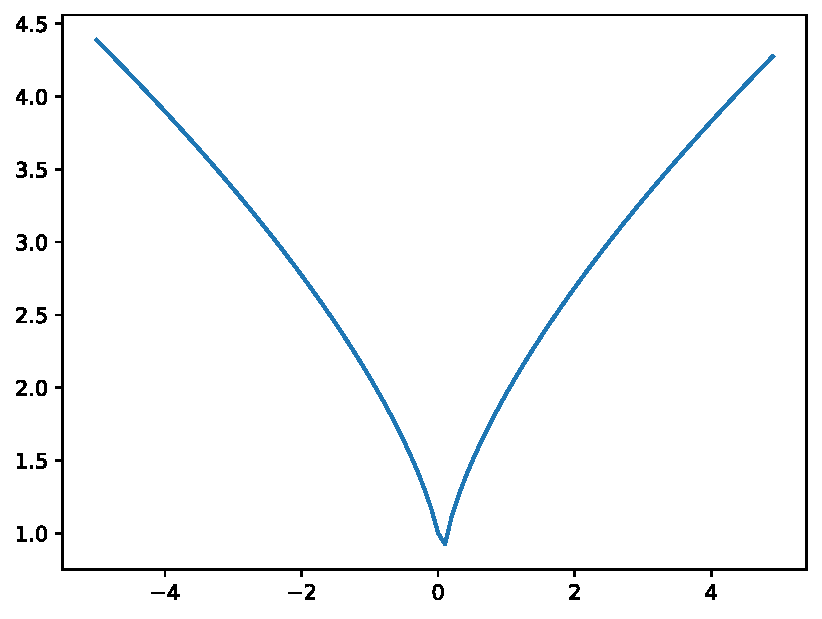
\includegraphics[width = .75\linewidth]{1.pdf}
						\caption[.] {График \( (5y-4)^{\frac{3}{2}} - 1 = 15x \)}
  					\end{figure}
			
				\item \(\begin{cases}
						2yy'' = 4y'^2 + y'',\\
						y(0) = 0, \\
						y'(0) = -2;
					\end{cases}\)
					
					\textit{Тип уравнения:} Общее уравнение несодержащее аргумента		

					\textit{Общее решение:} \( y = \dfrac{C_1x+C_2 - 1}{2(C_1x + C_2)} \)
	
					\textit{Задача Коши:} \( y = \dfrac{2x}{4x-1} \)

					\begin{figure}[H]
					   	\centering
					    	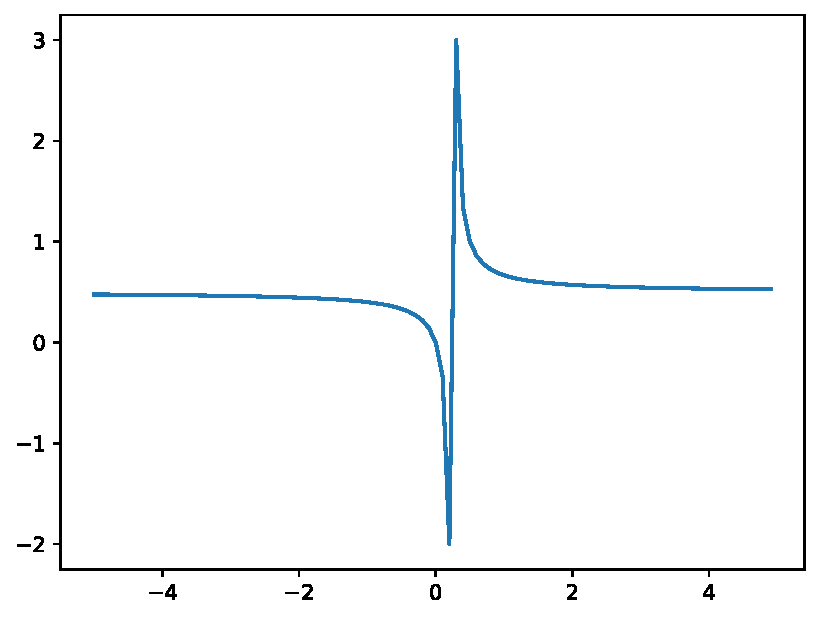
\includegraphics[width = .75\linewidth]{2.pdf}
						\caption[.] {График  \( y = \dfrac{2x}{4x-1} \)}
  					\end{figure}
			\end{enumerate}

	\pagebreak
	\section{Задание 3}
		\subsection{Постановка задачи}
			\noindent Дано логистическое уравнение популяции:
				\[ \dfrac{dP(t)}{dt} = kP(t) \cdot \bigg( 1- \dfrac{P(t)}{M}\bigg),\;\; \begin{matrix} P(0) = 800, &  \phantom{-}P(800) = 1100 \\ M = 29000, & P(t_i) = 3100 \end{matrix} \]
				Аналитически найти, при каких \(k\) и \(t_i\) решение будет удовлетворять условиям
				выше. Вывести соответствующую систему для неизвестных. Построить график
				решения данного уравнения. Решение оформить в среде \TeX .
		\subsection{Решение}
				\noindent Решим дифференциальное уравнение:
					\[ \dfrac{P}{M-P} = Ce^{kt} \]
				\noindent Составим систему для неизвестных и решим её:

					\[\begin {cases}
						\dfrac{800}{28200} = Ce^0, \\[7pt]
						\dfrac{1100}{27900} = Ce^{800k}, \\[7pt]
						\dfrac{3100}{25900} = Ce^{kt_i};
					\end {cases}\]
					
					\[\begin {cases}
						\dfrac{800}{28200} = C, \\[7pt]
						\ln{\bigg(\dfrac{1551}{1116}}\bigg)^{1/800} = k, \\[7pt]
						 \log_{\frac{1551}{1116}}\bigg({\dfrac{4371}{1036}}\bigg)^{800} = t_i.
					\end {cases}\]
			
					\begin{figure}[H]
					   	\centering
					    	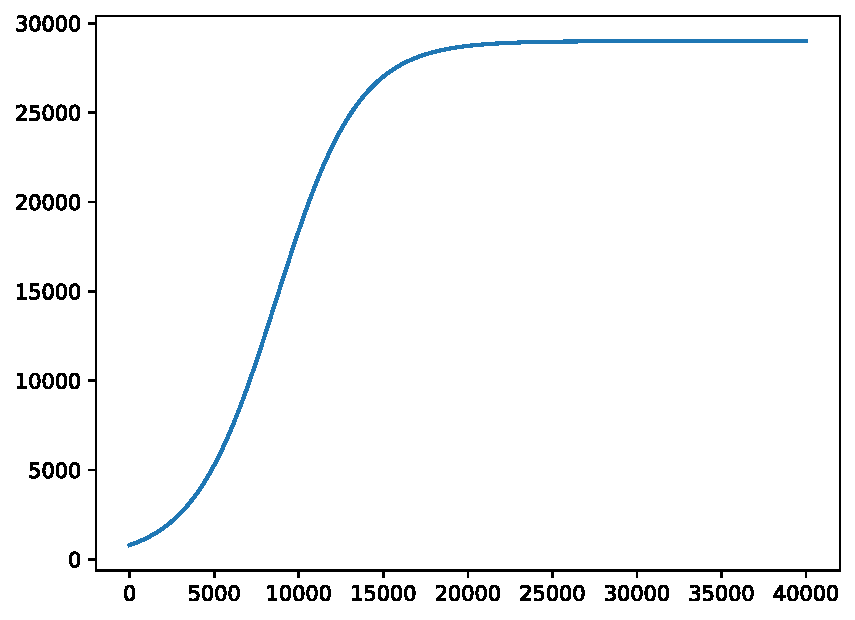
\includegraphics[width = .75\linewidth]{3.pdf}
						\caption[.] {График решения уравнения}
  					\end{figure}		
					
	\section{Заключение}
		\noindent Я решил 5 линейных уравнений высших порядков, 2 задачи Коши для уравнений 2-го порядка и аналитически нашёл коэффициент для логистического уравнения. Оформлял отчёт по работе в <<\TeX \:Live>>.
\end{document}	